\newpage
\section{Reading Information From a Graph}

On the next page is the graph of a function called $h(t)$, which
represents the distance (in miles) and direction (east = positive,
west = negative) Johnny is from home $t$ hours after noon. It does not
have a simple formula, so don't try to find one. Answer the following
questions about $h$, briefly explaining how you obtained your
answer(s):

\begin{prob}
On the given graph of $h$, what are the least and greatest values
of $t$? What are the greatest and least values of $h(t)$? What do
these answers say about Johnny?
\end{prob}

\begin{prob}
Evaluate the following expressions: $h(0)$, $h(3)$, and $h(-3)$. What
do each of these say about Johnny? 
\end{prob}

\begin{prob}
For each of the following, solve for $t$ (i.e., find all the values of
$t$ that make the statement true). Describe what you did with the
graph to determine the solutions.  Where possible, interpret
the statement and its solutions in terms of Johnny.

\begin{enumerate}
\item $h(t) = 0$
\item $h(t) = 3$
\item $h(t) \leq 3$
\item $h(t) = h(4.5)$
\item $h(t) = t$
\item $h(t) = -t$
\item $h(t) = h(-t)$
\item $h(t) = -h(-t)$
\item $h(t+1) = h(t)$
\item $h(t)+1 = h(t)$
\end{enumerate}
\end{prob}

\newpage

\[
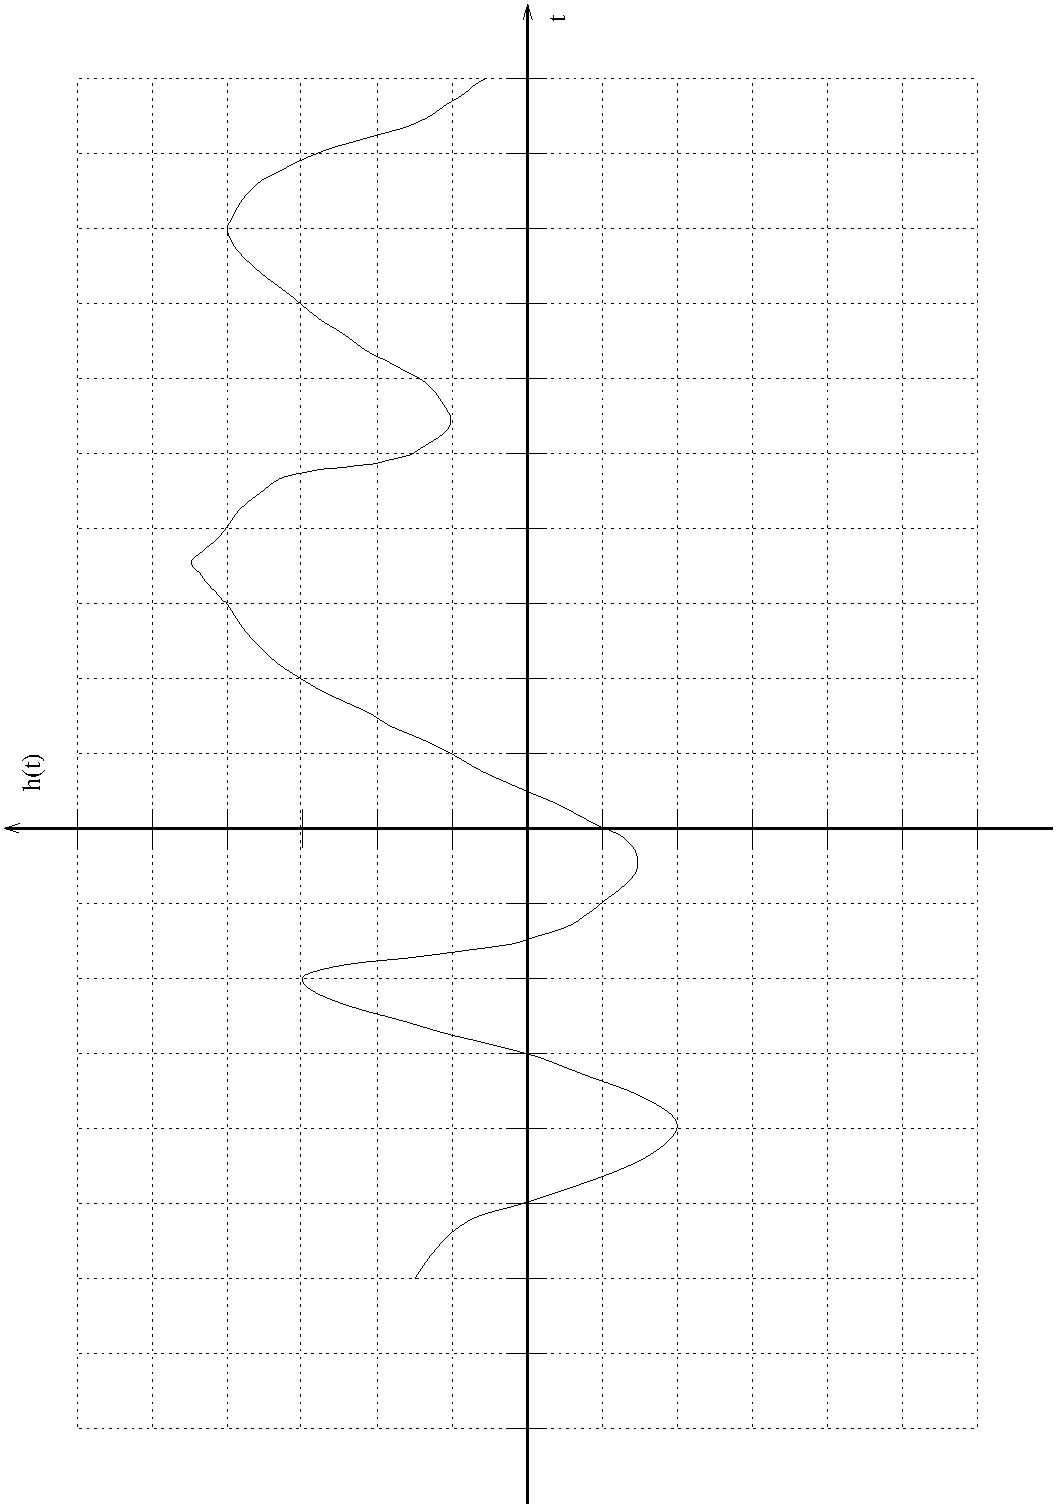
\includegraphics[scale=0.75]{../graphics/graphicDetails.pdf}
\]
